% Verze pro: LaTeX
% Verze hlavicky: 22. 2. 2007
% Autor: Ustav fyziky kondenzovanych latek
% Ke stazeni: www.physics.muni.cz/ufkl/Vyuka/
% Licence: volne k pouziti, nejlepe k vcasnemu odevzdani protokolu z Vaseho mereni.

\documentclass[a4paper,11pt]{article}

% Kodovani (cestiny) v dokumentu: cp1250
% \usepackage[cp1250]{inputenc}	% Omezena stredoevropska kodova stranka, pouze MSW.
\usepackage[utf8]{inputenc}	% Doporucujeme pouzivat UTF-8 (unicode).

%%% Nemente:
\usepackage[margin=2cm]{geometry}
\newtoks\jmenopraktika \newtoks\jmeno \newtoks\datum
\newtoks\obor \newtoks\skupina \newtoks\rocnik \newtoks\semestr
\newtoks\cisloulohy \newtoks\jmenoulohy
\newtoks\tlak \newtoks\teplota \newtoks\vlhkost
%%% Nemente - konec.


%%%%%%%%%%% Doplnte pozadovane polozky:

\jmenopraktika={Fyzikální praktikum 1}  % nahradte jmenem vaseho predmetu
\jmeno={Milan Suk}            % nahradte jmenem mericiho
\datum={9. března 2017}        % nahradte datem mereni ulohy
\obor={F}                     % nahradte zkratkou vami studovaneho oboru
\skupina={ČT 8:00}            % nahradte dobou vyuky vasi seminarni skupiny
\rocnik={I}                  % nahradte rocnikem, ve kterem studujete
\semestr={II}                 % nahradte semestrem, ve kterem studujete

\cisloulohy={2}               % nahradte cislem merene ulohy
\jmenoulohy={Měření odporu} % nahradte jmenem merene ulohy

\tlak={98,9}                   % nahradte tlakem pri mereni (v hPa)
\teplota={22,1}               % nahradte teplotou pri mereni (ve stupnich Celsia)
\vlhkost={50}               % nahradte vlhkosti vzduchu pri mereni (v %)

%%%%%%%%%%% Konec pozadovanych polozek.


%%%%%%%%%%% Uzitecne balicky:
\usepackage[czech]{babel}
\usepackage{graphicx}
\usepackage{amsmath}
\usepackage{xspace}
\usepackage{url}
\usepackage{indentfirst}

%%%%%% Zamezeni parchantu:
\widowpenalty 10000 \clubpenalty 10000 \displaywidowpenalty 10000
%%%%%% Parametry pro moznost vsazeni vetsiho poctu obrazku na stranku
\setcounter{topnumber}{3}	  % max. pocet floatu nahore (specifikace t)
\setcounter{bottomnumber}{3}	  % max. pocet floatu dole (specifikace b)
\setcounter{totalnumber}{6}	  % max. pocet floatu na strance celkem
\renewcommand\topfraction{0.9}	  % max podil stranky pro floaty nahore
\renewcommand\bottomfraction{0.9} % max podil stranky pro floaty dole
\renewcommand\textfraction{0.1}	  % min podil stranky, ktery musi obsahovat text
\intextsep=8mm \textfloatsep=8mm  %\intextsep pro ulozeni [h] floatu a \textfloatsep pro [b] or [t]

% Tecky za cisly sekci:
\renewcommand{\thesection}{\arabic{section}.}
\renewcommand{\thesubsection}{\thesection\arabic{subsection}.}
% Jednopismenna mezera mezi cislem a nazvem kapitoly:
\makeatletter \def\@seccntformat#1{\csname the#1\endcsname\hspace{1ex}} \makeatother


%%%%%%%%%%%%%%%%%%%%%%%%%%%%%%%%%%%%%%%%%%%%%%%%%%%%%%%%%%%%%%%%%%%%%%%%%%%%%%%
%%%%%%%%%%%%%%%%%%%%%%%%%%%%%%%%%%%%%%%%%%%%%%%%%%%%%%%%%%%%%%%%%%%%%%%%%%%%%%%
% Zacatek dokumentu
%%%%%%%%%%%%%%%%%%%%%%%%%%%%%%%%%%%%%%%%%%%%%%%%%%%%%%%%%%%%%%%%%%%%%%%%%%%%%%%
%%%%%%%%%%%%%%%%%%%%%%%%%%%%%%%%%%%%%%%%%%%%%%%%%%%%%%%%%%%%%%%%%%%%%%%%%%%%%%%

\begin{document}

%%%%%%%%%%%%%%%%%%%%%%%%%%%%%%%%%%%%%%%%%%%%%%%%%%%%%%%%%%%%%%%%%%%%%%%%%%%%%%%
% Nemente:
%%%%%%%%%%%%%%%%%%%%%%%%%%%%%%%%%%%%%%%%%%%%%%%%%%%%%%%%%%%%%%%%%%%%%%%%%%%%%%%
\thispagestyle{empty}

{
\begin{center}
\sf 
{\Large Ústav fyzikální elektroniky Přírodovědecké fakulty Masarykovy univerzity} \\
\bigskip
{\huge \bfseries FYZIKÁLNÍ PRAKTIKUM} \\
\bigskip
{\Large \the\jmenopraktika}
\end{center}

\bigskip

\sf
\noindent
\setlength{\arrayrulewidth}{1pt}
\begin{tabular*}{\textwidth}{@{\extracolsep{\fill}} l l}
\large {\bfseries Zpracoval:}  \the\jmeno & \large  {\bfseries Naměřeno:} \the\datum\\[2mm]
\large  {\bfseries Obor:} \the\obor  \hspace{40mm}  {\bfseries Skupina:} \the\skupina %
%{\bfseries Ročník:} \the\rocnik \hspace{5mm} {\bfseries Semestr:} \the\semestr  
&\large {\bfseries Testováno:}\\
\\
\hline
\end{tabular*}
}

\bigskip

{
\sf
\noindent \begin{tabular}{p{3cm} p{0.6\textwidth}}
\Large  Úloha č. {\bfseries \the\cisloulohy:} \par
\smallskip
$T=\the\teplota$~$^\circ$C \par
$p=\the\tlak$~hPa \par
$\varphi=\the\vlhkost$~\%
&\Large \bfseries \the\jmenoulohy  \\[2mm]
\end{tabular}
}

\vskip1cm

%%%%%%%%%%%%%%%%%%%%%%%%%%%%%%%%%%%%%%%%%%%%%%%%%%%%%%%%%%%%%%%%%%%%%%%%%%%%%%%
% konec Nemente.
%%%%%%%%%%%%%%%%%%%%%%%%%%%%%%%%%%%%%%%%%%%%%%%%%%%%%%%%%%%%%%%%%%%%%%%%%%%%%%%

%%%%%%%%%%%%%%%%%%%%%%%%%%%%%%%%%%%%%%%%%%%%%%%%%%%%%%%%%%%%%%%%%%%%%%%%%%%%%%%
%%%%%%%%%%%%%%%%%%%%%%%%%%%%%%%%%%%%%%%%%%%%%%%%%%%%%%%%%%%%%%%%%%%%%%%%%%%%%%%
% Zacatek textu vlastniho protokolu
%%%%%%%%%%%%%%%%%%%%%%%%%%%%%%%%%%%%%%%%%%%%%%%%%%%%%%%%%%%%%%%%%%%%%%%%%%%%%%%
%%%%%%%%%%%%%%%%%%%%%%%%%%%%%%%%%%%%%%%%%%%%%%%%%%%%%%%%%%%%%%%%%%%%%%%%%%%%%%%


\section{Úvod}

    \paragraph{} Cílem toho měření je
    
    \begin{enumerate}
        \item zjistit odpor rezistoru pomocí měření napětí a proudu a s použitím Ohmova zákona.
        \item změřit volampérovou charakteristiku žárovky
    \end{enumerate}

\section{Postup měření}

    \subsection{Metoda A}

        \paragraph{} U metody A je změřeným napětí $U$ správné napětí na rezistoru, ale 
        měřený proud je roven součtu proudu $I_{R}$, takoucího rezistorem, a $I_{A}$,
        který protéká ampérmetrem. Pro hledaný odpor platí

        \begin{equation} 
            R = \frac{U}{I_{A} - \frac{U}{R_{V}}}
        \end{equation}

        kde $R_{V}$ je odpor voltmetru.
        
        \begin{figure}[h]
            \centering
            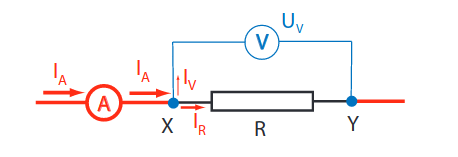
\includegraphics[width=0.6\textwidth]{metoda_a.png}
            \caption{Schéma k metodě A}
            \label{fig:method_a}
        \end{figure}

    \subsection{Metoda B}

        \paragraph{} Při zapojení metodou B měříme správný proud $I_{A}$, který se shoduje
        s proudem na rezistoru, ale zato změřené napětí je dáno součtem napětí na ampérmetru
        a rezistoru. Zde pro hledanou hodnotu odporu platí

        \begin{equation}
            R = \frac{U_{V} - R_{A} I_{A}}{I_{A}}
        \end{equation}

        kde $R_{A}$ je odpor ampérmetru.
        
        \begin{figure}[h]
            \centering
            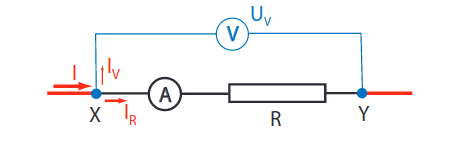
\includegraphics[width=0.6\textwidth]{metoda_b.png}
            \caption{Schéma k metodě B}
            \label{fig:method_b}
        \end{figure}

    \subsection{Měření voltampérové charakteristiky žárovky}

        \paragraph{} Nakonec měření voltampérové charakteristiky žárovky provádíme
        pomocí zapojení A a postupně měříme dvojici (napětí [$mA$], proud [$V$]), přičemž 
        napětí na zdroji volíme v rozmezí od $U = 0V$ do $U = 20V$. 

\section{Výsledky}

    \paragraph{} Velikost odporu ampérmetru při rozsahu do $400 mA$ činí

    \begin{equation}
        R_{A} = 1.165 \Omega
    \end{equation}

    a odpor volmetru je

    \begin{equation}
        R_{V} = 11.1 M\Omega
    \end{equation}

    \subsection{Metoda A}

        \begin{table}[h]
            \centering
            \begin{tabular}{ | l || l | l || l | }
                \hline
                        & $U$ $[V]$ & $I$ $[mA]$             & $R$ $[\Omega]$    \\ \hline
                $R_{1A}$ & $20.51$   & $199.2$               & $102.9628 \pm 0.07$         \\ \hline
                $R_{2A}$ & $20.92$   & $21.7 \cdot 10^{-3}$  & $1055749.0339 \pm 0.7$      \\
                \hline
            \end{tabular}
            \caption{Měření odporů metodou A}
            \label{fig:method_b}
        \end{table}

        \paragraph{} Nepřesnost měření je podle principu šíření nejistot

        \begin{equation}
            u(R_{A}) = \frac{\sqrt{I^{2} u^{2}(U) + U^{2} u^{2}(I)}}{(I - \frac{U}{R_{V}})^{2}}
        \end{equation}

        \paragraph{}

    \subsection{Metoda B}

        \begin{table}[h]
            \centering
            \begin{tabular}{ | l || l | l || l | }
                \hline
                        & $U$ $[V]$ & $I$ $[mA]$             & $R$ $[\Omega]$     \\ \hline
                $R_{1B}$ & $23.01$   & $208.5$               & $109.19 \pm 0.07$  \\ \hline
                $R_{2B}$ & $19.92$   & $19.9 \cdot 10^{-3}$  & $1000904.9 \pm 0.7$\\
                \hline
            \end{tabular}
            \caption{Měření odporů metodou A}
            \label{fig:method_b}
        \end{table}

        \paragraph{} Zde je nepřesnost měření podle principu šíření nejistot

        \begin{equation}
            u(R_{B}) = \frac{\sqrt{I^{2} u^{2}(U) + U^{2} u^{2}(I)}}{I^{2}}
        \end{equation}

    \subsection{Měření voltampérové charakteristiky žárovky}

        \begin{figure}[h]
            \centering
            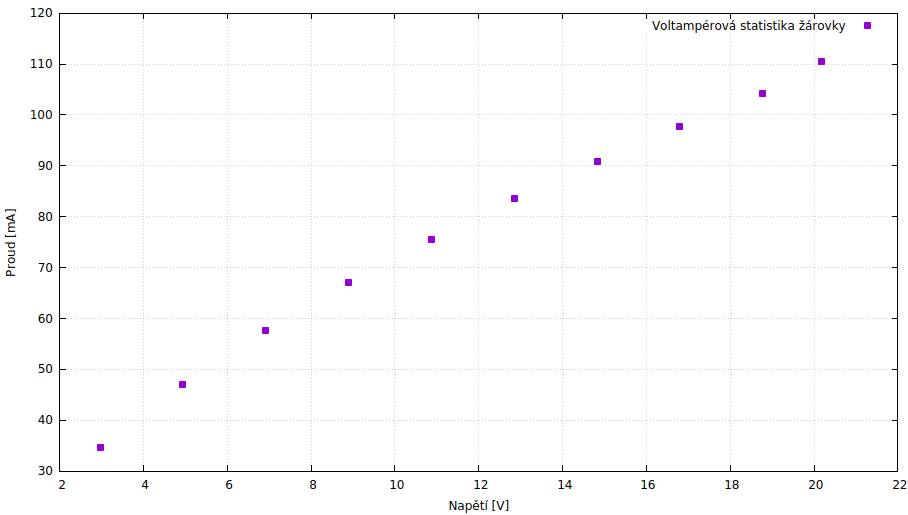
\includegraphics[width=0.8\textwidth]{zarovka1.png}
            \caption{Voltapmérová charakteristika žárovky}
            \label{fig:zarovka}
        \end{figure}

        \paragraph{}

    \section{Zhodnocení měření, závěr}

    \paragraph{} 

        \begin{table}[h]
            \centering
            \begin{tabular}{ | l | l | }
                \hline
                         & $R$                  \\ \hline
                $R_{1A}$ & 102.9628             \\ \hline
                $R_{2A}$ & 1055749.0339         \\ \hline
                $R_{1B}$ & 109.1947             \\ \hline
                $R_{2B}$ & 1000904.9251         \\
                \hline
            \end{tabular}
            \caption{Měření odporů metodou A}
            \label{fig:method_b}
        \end{table}
\end{document}

